\chapter{Conclusion}
\label{chap:conclusion}

In this thesis, we have successfully developed an HTML read-only Integrated Development Environment (IDE) for the Rust programming language \cite{sevenzing_2023_8017323}. The aim of the tool was to provide a comprehensive code visualization functionality to aid developers in quickly understanding and comprehending Rust code. We have achieved this goal by leveraging the popular features of existing solutions in the field of Rust code text visualization, such as syntax highlighting, cross-entity links, and displaying information about declaration and usage. However, unlike existing solutions, our tool focuses on providing cross-platform portability by generating a single HTML file report.

The development process involved extensive research on the Rust programming language and existing solutions for Rust code text visualization. We designed and implemented the tool, considering the requirements of handling large and complex codebases without proper documentation. The tool has been tested for various use cases, ensuring its functionality and usability.

By releasing the first version of our tool, we have covered all the initial requirements \ref{table:must_req} and provided a valuable resource for developers, project managers, stakeholders, researchers, and educators in the Rust community. The HTML report offers an efficient and convenient way to navigate and comprehend Rust code, facilitating code review, project assessment, and language exploration.

\section{Results}

To evaluate the effectiveness and performance of our HTML report for Rust, we conducted several metric-based analyses. The results provide insights into the tool's capabilities and limitations. Table \ref{table:metrics} presents the metrics obtained from analyzing different projects.

We conducted a thorough analysis of the metrics to evaluate the effectiveness and efficiency of our HTML report for Rust. One of the key metrics we considered was the comparison between the size of the target project and the size of the generated HTML report. This metric provides insights into the level of information and code coverage provided by our tool.

By comparing the number of lines of code, we obtained a quantitative measure of the amount of code represented in the target project and the resulting HTML report. This comparison helps assess the comprehensiveness of the report and its ability to capture the essential aspects of the project.

Furthermore, we examined the project size versus the report size in terms of disk space. This metric provides an understanding of the file size reduction achieved by generating the HTML report. A smaller report size not only makes the file more portable and easier to share but also improves the overall accessibility and convenience of the tool.

In addition to evaluating the size metrics, we measured the time required to build the HTML report. The experiment was conducted utilizing the Apple M1 chip, equipped with 16GB of RAM. This performance metric is crucial in determining the efficiency of our tool. While the report generation process took a significant amount of time, approximately 120 seconds, it is important to consider the complexity and size of the project being analyzed. The comprehensive analysis and indexing of project dependencies are necessary steps for accurate code visualization and cross-entity linking.

\begin{longtable}{| p{0.7cm} | p{2cm} | p{2.5cm} | p{2.5cm} | p{3cm} | p{3cm}| }
\caption[Project metrics]{Project metrics} \label{table:metrics} \\
\hline
\# & Time to run generator & Lines in project & Lines in report  &  Project size  & Report size \\
\endfirsthead
\endhead
\hline
\href{https://github.com/sevenzing/test-rust-crate/tree/master}{1} & 54s & 273 & 582 & 44 KBytes & 184 KBytes \\
 \hline
\href{https://github.com/sevenzing/thesis}{2} & 2m 26s & 920 & 1715 & 272 Kbytes & 1,4 MBytes \\
 \hline
\href{https://github.com/blockscout/blockscout-rs/tree/main/stats}{3} & 4m 48s & 5562 & 7569 & 832 KBytes & 3,6 Mbytes \\
 \hline
\href{https://github.com/blockscout/blockscout-rs/tree/main/smart-contract-verifier}{4} & 5m 23s & 14404 & 15,994 & 1,9 Mbytes & 13 Mbytes \\
 \hline
\end{longtable}

From the metrics, we can observe that the time to build the reports increases as the complexity and size of the projects grow. Generating a comprehensive HTML report requires significant time due to the need to index all the dependencies of the project accurately. The size of the reports also increases proportionally with the size of the projects, as more code and information need to be included.

These metrics indicate that report generation, especially for larger projects, may take considerable time. While this poses a challenge, there is no simple solution to expedite the process since accurately indexing dependencies is crucial for the comprehensiveness of the report. Future optimizations and improvements may be explored to enhance the efficiency of report generation.

\section{System Demonstration}

This section showcases the functionality and operation of the implemented thesis project. It includes a series of screenshots accompanied by concise descriptions, providing an illustrative overview of the system's key features and user interactions. 

Fig. \ref{fig:initial} illustrates the initial interface of the report, which consists of a divided window upon opening. The left section displays a project tree, while the right section showcases a code area. The gray separator between the project tree and the code section can be moved to customize the width of the project tree for convenient customization. Upon clicking on files within the project tree, the corresponding file content is displayed in the code section. 


\begin{figure}[ht]
\centering
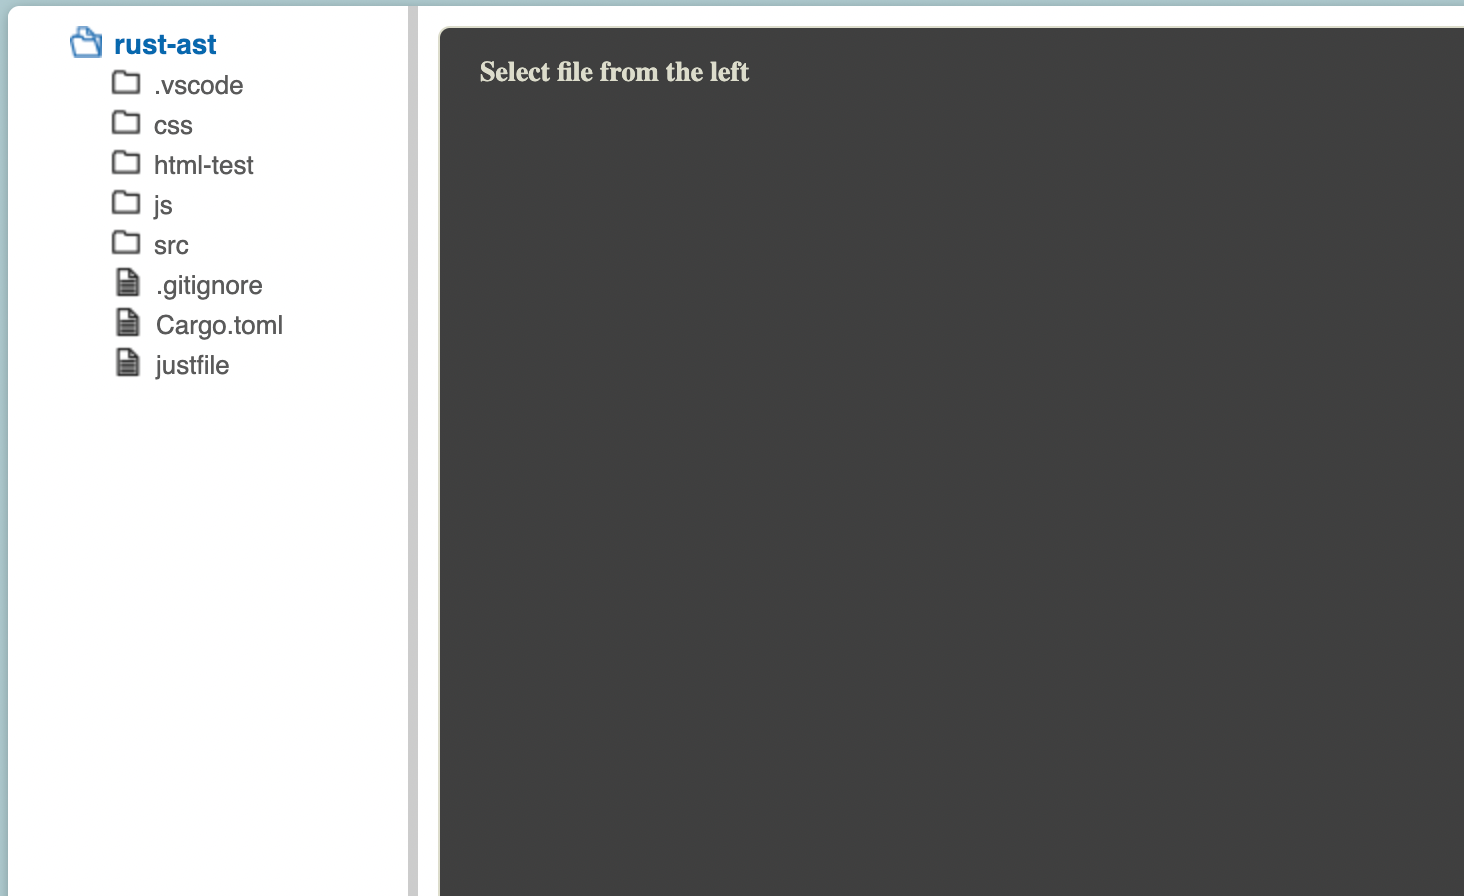
\includegraphics[width=15cm]{figs/screenshots/initial.png}
\caption{Initial content of the report.}
\label{fig:initial}
\end{figure}


Upon clicking on a file name in the project tree, the top section of the code will display the name of the current file, and the highlighted content of the file will be rendered. When hovering over a variable, function, or expression, the user is presented with additional information such as the final type, function signature, or module information. An example of such hover information can be seen in Fig. \ref{fig:hover}.

\begin{figure}[ht]
\centering
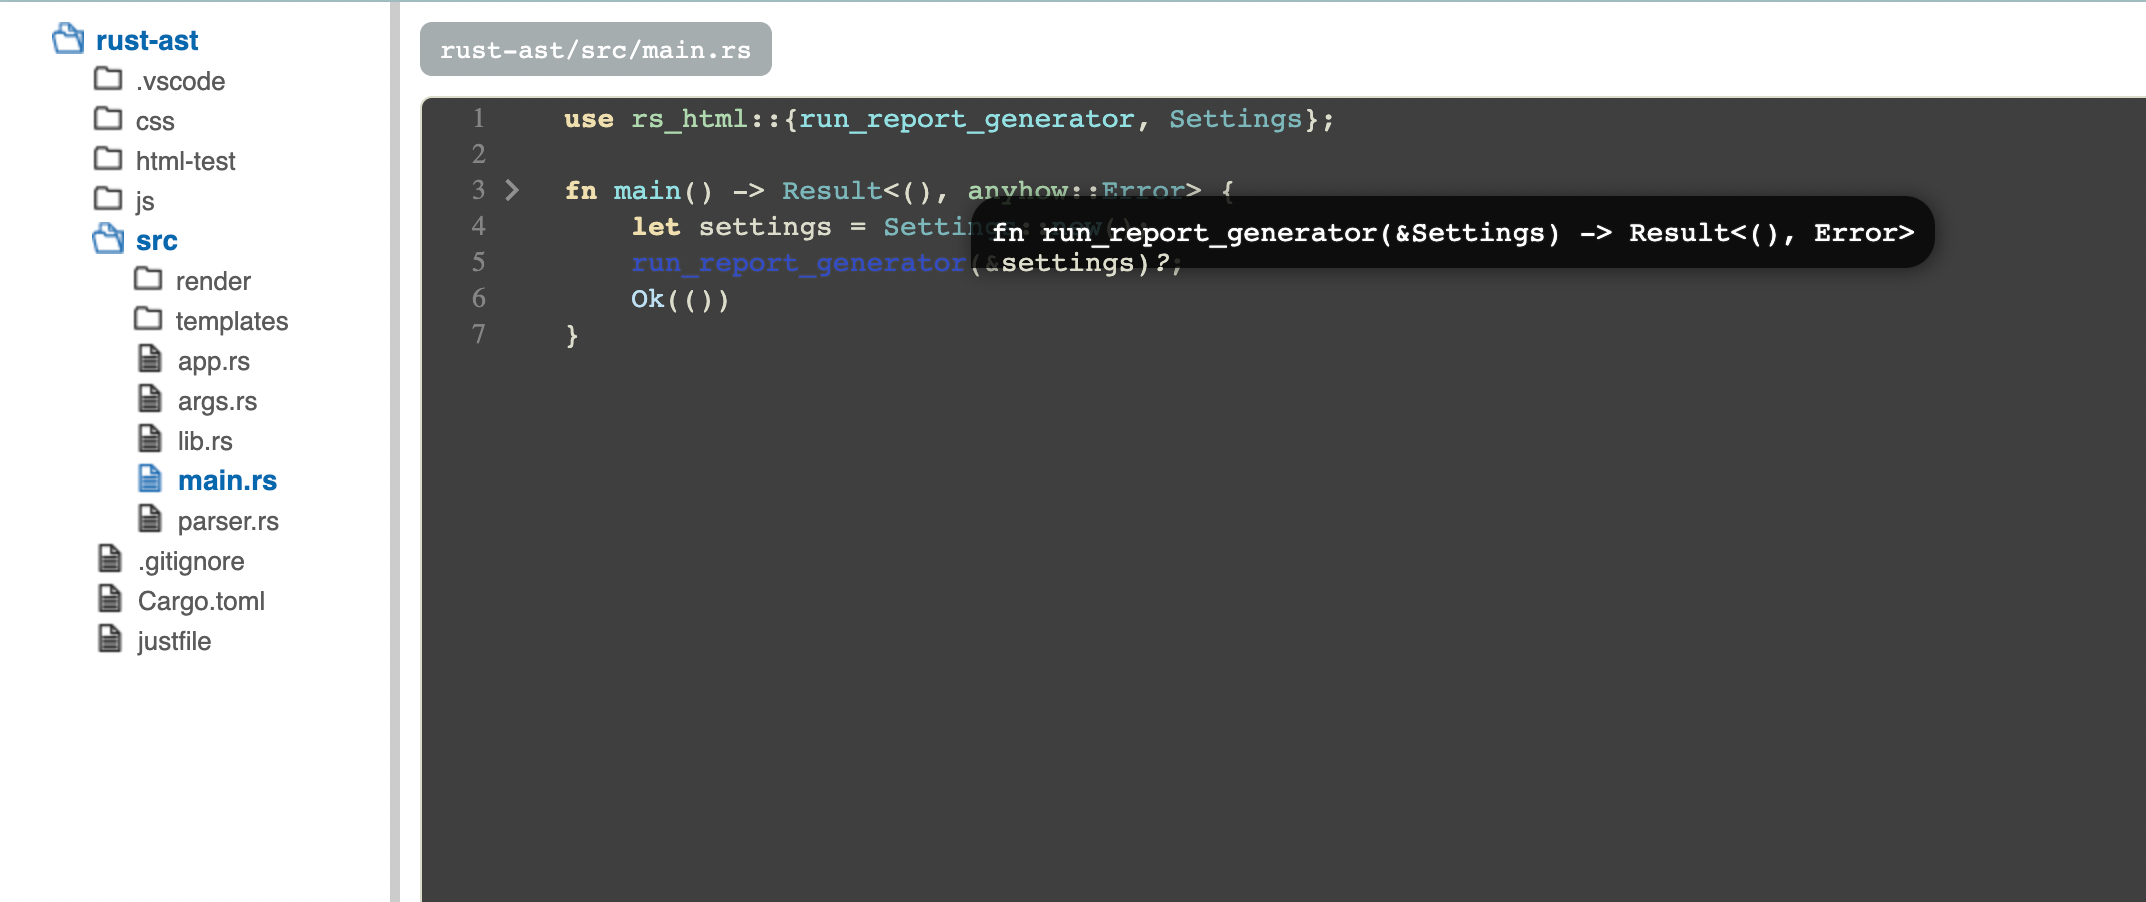
\includegraphics[width=15cm]{figs/screenshots/hover.png}
\caption{Additional information when user cursors token.}
\label{fig:hover}
\end{figure}

When holding down the meta key on the keyboard (\textbf{Cmd} in macOS, \textbf{Ctrl} in Windows and Linux) and clicking on a variable, function, structure, etc., near the clicked location, a navigation menu opens with two tabs. Fig. \ref{fig:nav_def} illustrates the "Definition" tab, which displays the declaration location of the object. Fig. \ref{fig:nav_refs} shows the "References" tab, which lists the places where this object is used. Clicking on a definition or reference location will jump to the desired location, with the necessary line highlighted. As depicted in Fig. \ref{fig:nav_refs}, the yellow background highlights line number 8, serving as a visual indication of the recent jump.

\begin{figure}[ht]
\centering
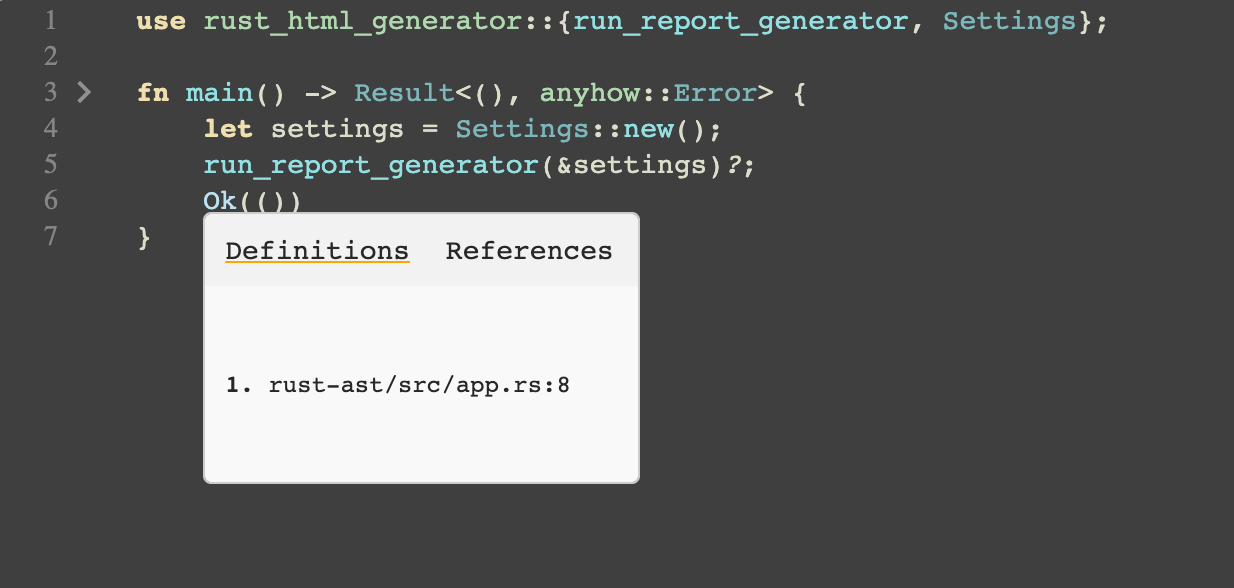
\includegraphics[width=15cm]{figs/screenshots/nav_def_2.png}
\caption{Navigation menu. Definition section.}
\label{fig:nav_def}
\end{figure}


\begin{figure}[ht]
\centering
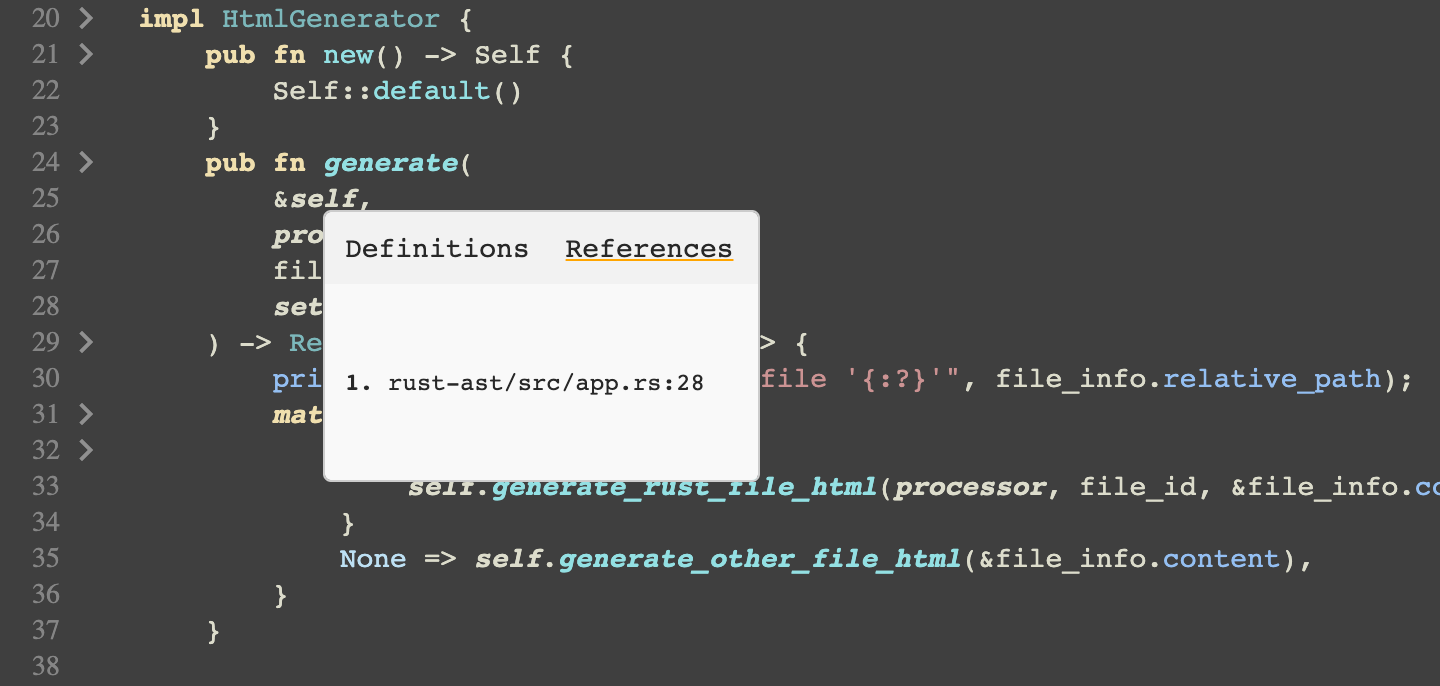
\includegraphics[width=15cm]{figs/screenshots/nav_refs_2.png}
\caption{Navigation menu. References section.}
\label{fig:nav_refs}
\end{figure}

Another beneficial aspect of a report is the ability to collapse or fold lines. This functionality is evident in Fig. \ref{fig:fold}, where each foldable line is accompanied by a right-facing arrow that can be clicked. When pressed, the arrow collapses the lines associated with the corresponding block, including function definitions, function signatures, if statements, match statements, and similar elements.

\begin{figure}[ht]
\centering
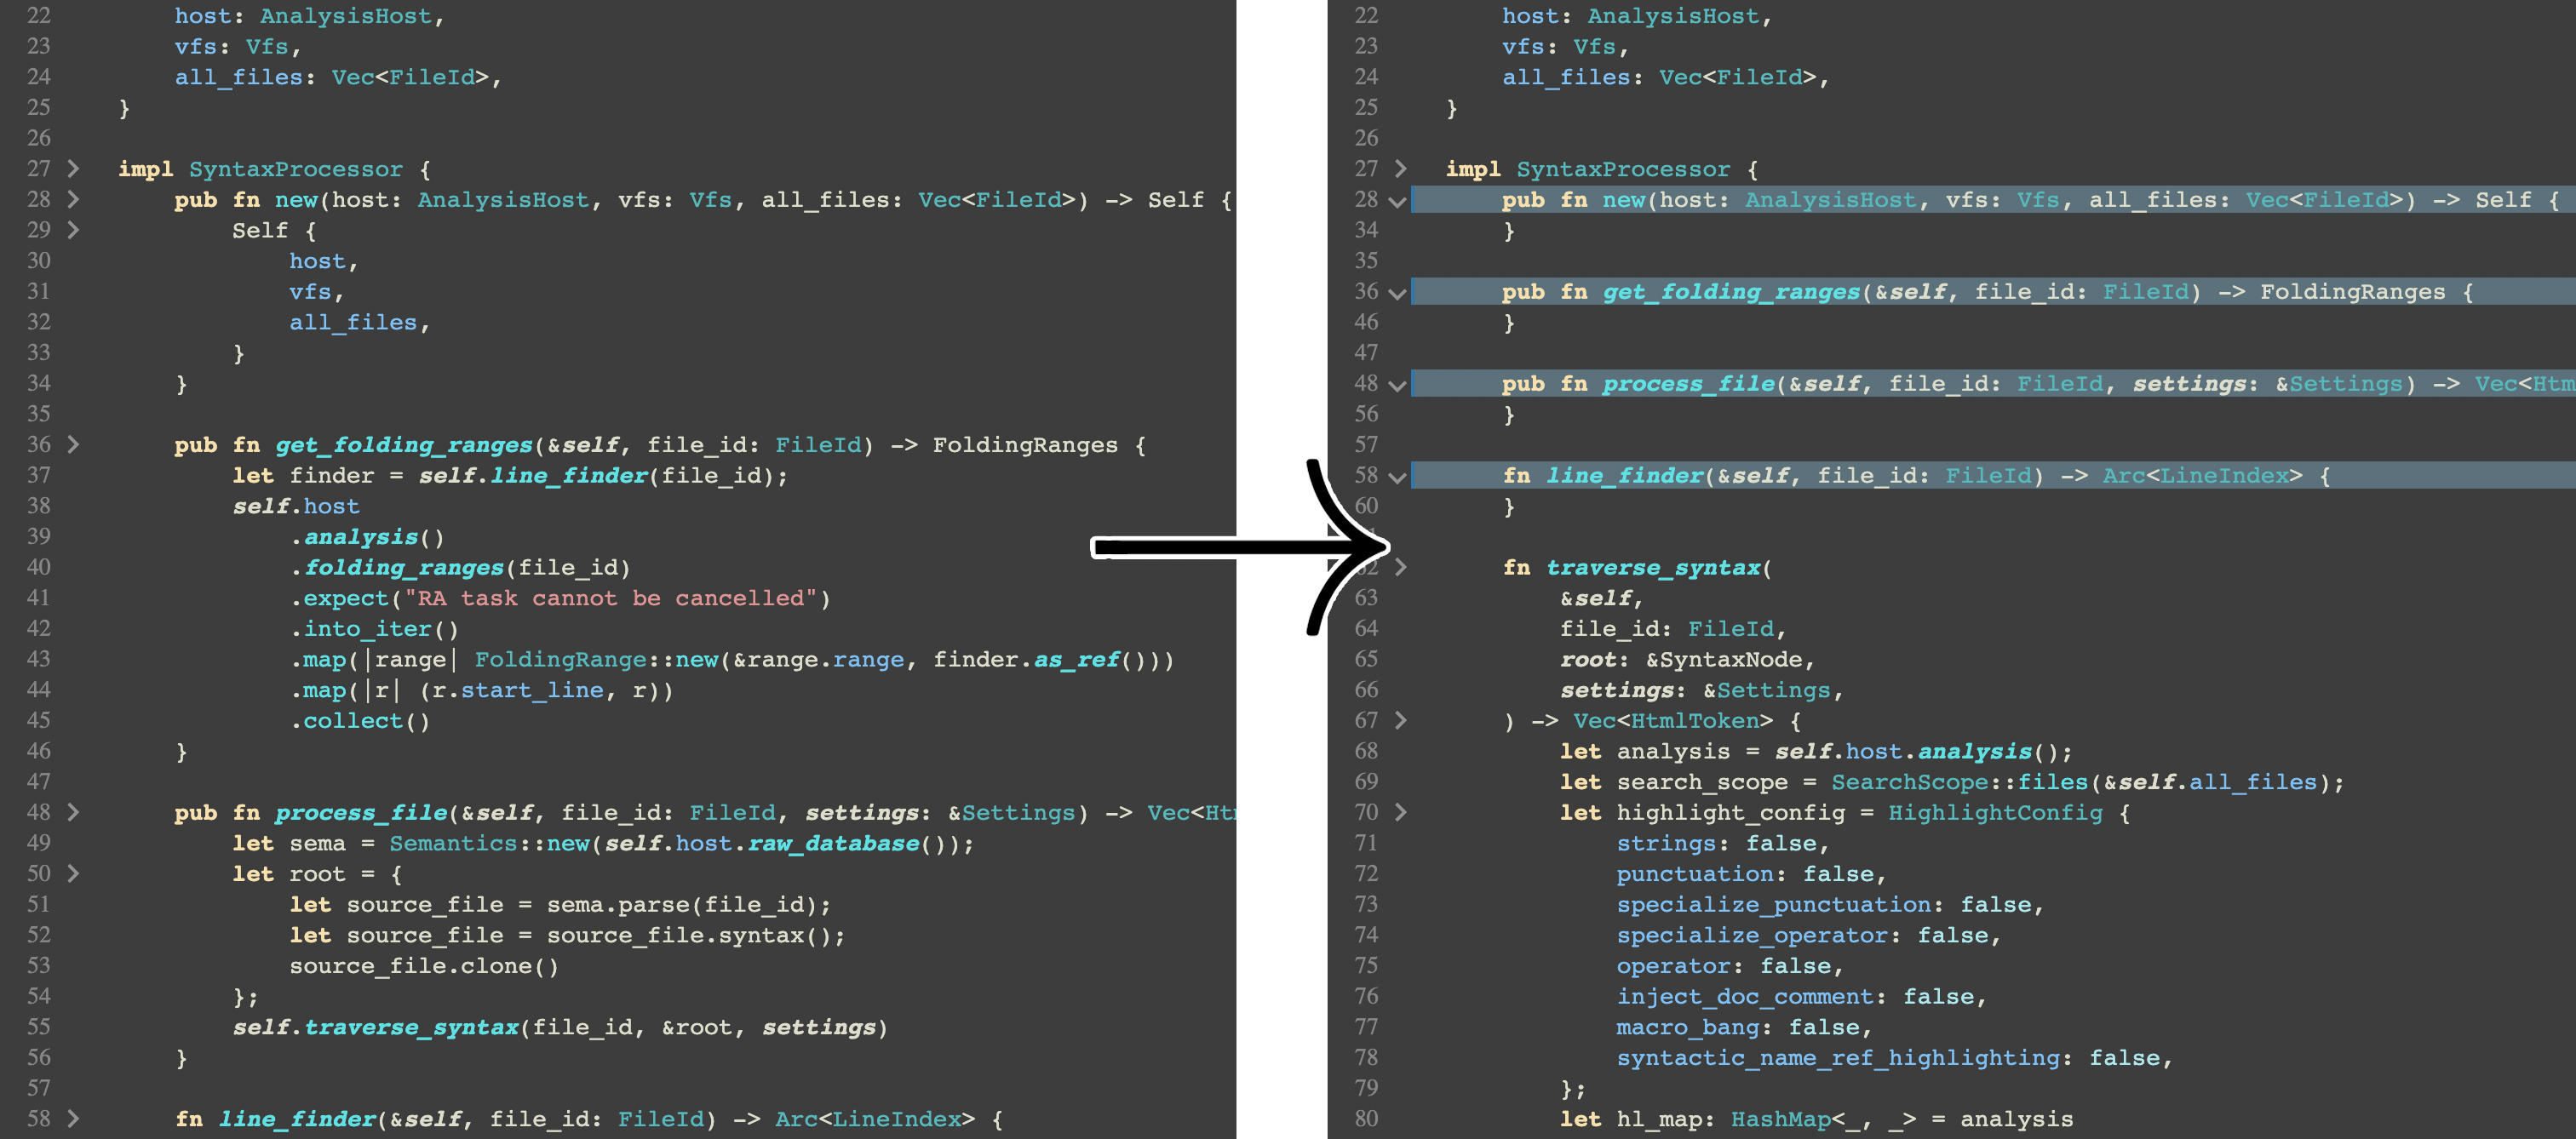
\includegraphics[width=15cm]{figs/screenshots/fold.png}
\caption{Collapsing (folding) code blocks.}
\label{fig:fold}
\end{figure}

\section{Future Work}

We have successfully accomplished our initial objectives and produced a fully operational system. Nevertheless, there exist numerous prospects for future endeavors and enhancements, which are as follows:

\begin{enumerate}
\item \textbf{Customizable Style Themes:} The incorporation of customizable style themes into the system would empower users to personalize the visual representation of Rust code within the HTML report. By introducing this feature, we would augment the overall user experience and cater to the individual preferences and requirements of users.

\item \textbf{Project Search:} The implementation of a project search functionality within the HTML report would furnish users with the ability to swiftly locate specific code snippets, functions, or variables. This notable addition would significantly ameliorate the navigability and accessibility of large-scale projects.

\item \textbf{Synchronization Problem:} Upon the completion of the report, it ceases to remain synchronized with the latest version of the project, as it incorporates the content of all files for the sake of portability. In order to address this issue, we propose the inclusion of an optional button that enables the synchronization of the current project version using a remote git repository.
\end{enumerate}